%!TEX root = pfc-memoria.tex
%!TEX encoding = UTF-8 Unicode


\section{Clasificadores}

\subsection{Bondad del clasificador (valor-F)}

Para la comparación de sistemas de búsqueda y recuperación de información disponemos de una métrica llamada valor-F\index{valor-F} (\emph{F-score}\index{F-score@\emph{F-score}}, \emph{F-measure}\index{F-measure@\emph{F-measure}} ó \emph{$F_1$ score}\index{F\_1 score@$F_1$ score}) siendo ésta la media armónica de otros dos indicadores: \citep{wikipedia:precision-exhaustividad}
\begin{description}
\item[precisión \emph{(precision)}] \index{precisión}\index{precision@\emph{precision}}
Es la fracción de instancias recuperadas que son relevantes.
\begin{eqnarray}
\text{precisión} &=& \frac{|\{\text{relevantes}\}\cap\{\text{recuperados}\}|}{|\{\text{recuperados}\}|}
\end{eqnarray}
\item[exhaustividad \emph{(recall)}] \index{exhaustividad}\index{recall@\emph{recall}}
Es la fracción de instancias relevantes que han sido recuperadas.
\begin{eqnarray}
\text{exhaustividad} &=& \frac{|\{\text{relevantes}\}\cap\{\text{recuperados}\}|}{|\{\text{relevantes}\}|}
\end{eqnarray}
\item[valor-F \emph{(F-score)}] Media armónica de precisión y exhaustividad.
\begin{eqnarray}
F_1 &=& 2\times\frac{\text{precisión}\times\text{exhaustividad}}{\text{precisión}+\text{exhaustividad}}
\end{eqnarray}
\end{description}

Supongamos un clasificador binario:
\begin{itemize}
\item La medida de precisión será el porcentaje de documentos correctamente clasificados dentro del conjunto de prueba.
\item La medida de exhaustividad será el porcentaje de documentos del conjunto de referencia que han sido correctamente clasificados. \citep{Perkins2010}
\end{itemize}


\section{Rendimiento en Python}

Se observó que la carga del modelo entrenado \path{GoogleNews-vectors-negative300.bin.gz} consumía mucho tiempo y espacio ($\approx$\si{4.5}{GiB} y unos 5 minutos). Este modelo ha sido publicado por Google en el repositorio del proyecto \code!word2vec! basado en el \emph{dataset} de Google News (aproximadamente 100 mil millones de palabras). El modelo contiene vectores 300-dimensionales para 3 millones de palabras y de frases (bigramas y trigramas). Las frases se obtuvieron usando una aproximación dirigida por datos sencilla, como se encuentra descrito en \cite{DBLP:journals/corr/MikolovSCCD13}.

Por ello se convirtió inicialmente el modelo del \emph{Word2Vec} original en la representación interna provista por \code!gensim!, que soporta en \emph{unpickling} de datos de NumPy, de mejor desempeño.

El procedimiento para la conversión es:

\begin{minted}{python}
from gensim.models.word2vec import Word2Vec
# lectura sin optimizar
model_orig = Word2Vec.load_word2vec_format('GoogleNews-vectors-negative300.bin', binary=True)
# escritura optimizada
model_orig.save('GoogleNews-vectors-negative300.bin.gensim')
\end{minted}

Y para la carga de la versión optimizada:

\begin{minted}{python}
from gensim.models.word2vec import Word2Vec
# lectura optimizada
model = Word2Vec.load('GoogleNews-vectors-negative300.bin.gensim', mmap='r')
\end{minted}


%\part{Introducción y objetivos}

%\chapter{Introducción}

%\chapter{Objetivos del proyecto}

%\chapter{Estructura de la memoria}

%\part{Estudio de viabilidad}

%\chapter{Metodología de trabajo}

%\chapter{Planificación temporal}

%\chapter{Análisis del esfuerzo de desarrollo}

%\part{Desarrollo del proyecto}

%\chapter{Análisis de requisitos}

\resizebox{0.5\textwidth}{!}{\input{diag1.puml}}

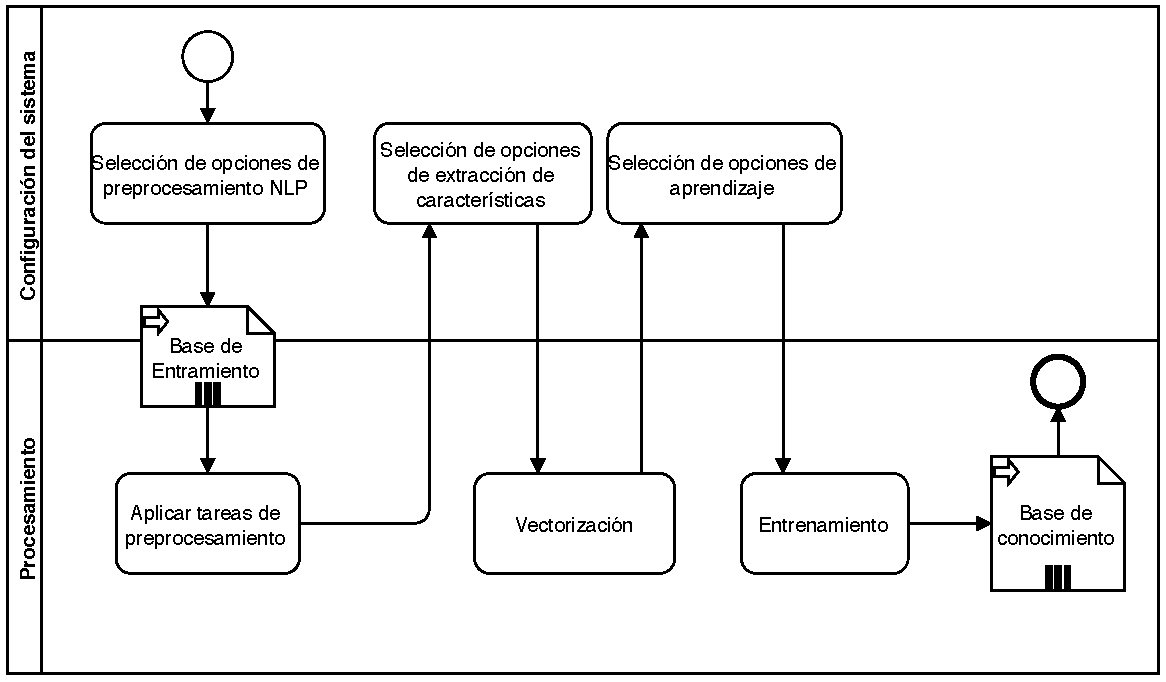
\includegraphics[width=\textwidth]{bpmn-entrenamiento}

%\chapter{Diseño del sistema}

%\chapter{Implementación}

%\part{Aseguramiento de la calidad}

%\chapter{Plan de pruebas}

%\chapter{Plan de mantenimiento}

%\part{Conclusiones}

%\chapter{Conclusiones}

\part{Apéndices}
\appendix

\chapter{Manual de usuario}

%bibliografía